\chapter{Related Work}

Today's use of the Internet is heavily based on content dissemination of all kinds of media like audio and video. TV-Shows, clips and tutorials on Youtube, podcasting for educational purposes like on Coursera need to be distributed around the globe. Popular TV-Shows are being often distributed globally within the first few hours after being telecast to the audience through p2p networks. If such a TV-Show reaches a certain attraction, it may be downloaded over 1.5 million times resulting in a transfer of almost 2'000 terabytes in the first 12 hours of being available \cite{forbes14}. In 2008 alone 500 exabytes were created and today's number is a multiple of that \cite{gantz07}. This became possible since computers and computing devices got so inexpensive that almost anybody can afford them. Limited storage on clouds is given free to all users by many providers. When the Internet was invented, there were only a few computers and few resources like tape storage devices, archives or computing power distributed geographically. A client requested some specific information or resources from a specific destination which needed to be known to the client. The client was connected through TCP/IP to the server, and after the connection was established and possibly secured, the transfer of the information needed by the client could start. Host-centric networking was very reasonable at that time, but the Internet evolved towards content-dissemination and with its evolution the need for new and more efficient solutions.

\vspace{5mm} %5mm vertical space

TCP/IP is no longer best suited for today's use of the Internet. One of the main reasons is that a TCP/IP connection is established between two machines and requires this connection to be active at all times. For content dissemination, a mechanism that supports multipoint to multipoint connections that do not have to be active at all times might be much better. Another reason is that a client often does not know where to get some specific information from (and doesn't really care) but knows exactly what it wants. Therefore a paradigm shift from host-centric networks started to evolve towards content-centric networks.

\newpage

\section{Named Data Network / Content Centric Networks}

Information-centric networking (ICN) is a possible answer to today's problems with TCP/IP architecture. ICN originated as a possible new paradigm for the future Internet to improve on scalability, reliability and efficient content distribution \cite{jacobson09, ndn17}. One of the many ICN architectures is content-centric networking (CCN) originally introduced by Van Jacobson. It is being continuously researched around the globe and one initiative trying to implement CCN is Named Data Networking (NDN) project.

\vspace{5mm} %5mm vertical space

In CCN the content is made directly addressable and routable by name. An Interest (request by a client) is sent out and routed according to its name until it reaches some endpoint that is able to respond with Content Objects to that Interest. Some of the main goals of CCN is better utilization of the bandwidth by increasing throughput and decreasing network traffic, better security, availability, flexibility and scalability of the networks. Better utilization of the bandwidth can be achieved by multicasting the same content to several endpoints and not re-unicasting the same content over and over again through the same channels near the content source. Also, content caching in intermediate nodes reduces the strain on bandwidth and increases overall efficiency. Better security is achieved by hashing and signing the content itself instead of the point-to-point connection between two hosts. Encrypting the data leads to more privacy within the Internet and could substitute many current access policy patterns used by servers and web pages. Better availability and flexibility are intrinsically given by content caching. Better scalability is achieved by not needing pre-planned structures like content delivery and P2P networks. Data is not only kept at the content producer but everywhere along the route if necessary.

\vspace{5mm} %5mm vertical space

\begin{figure}[H]
  \centering
  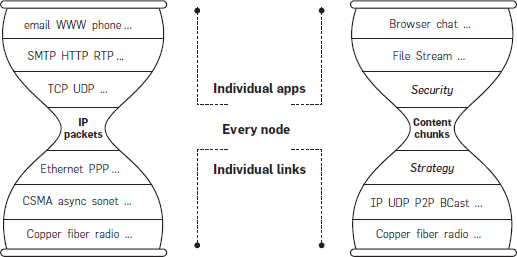
\includegraphics[scale=0.6]{chapter-2/NetworkStack}
  \caption{TCP/IP protocol stack on the left and CCN protocol stack on the right \cite{jacobson09}.}
  \label{fig:NetworkStack}
\end{figure}

\newpage

In Figure \ref{fig:NetworkStack} the IP and CCN protocol stacks are compared to each other. Both protocol stacks are built in a modular fashion that makes the architecture very flexible and scalable. The thin waste of the TCP/IP protocol stack consists of IP packages that have a source and a destination address. This Internet Layer is kept very simple and it makes only very weak demands on the lower Network Access Layer. This thin waist in TCP/IP protocol stack (\emph{where}) is replaced in CCN with a content layer (\emph{what}) that describes what the package is and has even fewer demands on the lower layer, keeping much of the advantages from IP. Lower layers of the CCN protocol stack are responsible for the routing, encoding and decoding of the information, while the higher layers consist of security and interpretation of the information. Because of the modularity, CCN can be implemented on top of IP.

\vspace{5mm} %5mm vertical space

Two big differences of TCP/IP and CNN are the strategy layer and the security layer. The strategy layer is responsible for all dynamic routing decisions based on the name and the strategy. The strategy can be a different one for different namespaces. E.g. an emergency message could be always broadcast according to its name. The Security layer differs from the TCP/IP protocol stack since the content chunks are signed and encrypted themselves, contrary to TCP/IP, where the connection is secured.

\subsection{CCN/NDN Node Model}

In CCN there are no clients and servers anymore but \textbf{consumers} and \textbf{producers}. Consumers request some information by sending out an \textbf{interest}. This interest packet consists of a content name, some selectors and a nonce. The interest is being forwarded according to the node's strategy until it reaches a node that can satisfy it. If a node can satisfy the received interest, it will respond with a \textbf{data} package consisting of the same content name as the interest, a signature, signed info and the data. The data will be sent back towards the consumer. The node having the requested information is called producer (it generates the data). Interests and data are received and sent out through interfaces which can be network or application interfaces.

\vspace{5mm} %5mm vertical space

\begin{figure}[H]
  \centering
  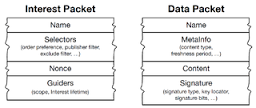
\includegraphics[scale=0.55]{chapter-2/InterestAndData}
  \caption{Overview of the packet structure for interests and data messages in NDN \cite{ndnWiki}.}
  \label{fig:InterestAndData}
\end{figure}

\vspace{5mm} %5mm vertical space

The most important data structures for routing the interest to the producer and the data back to the consumer are called the pending interest table (PIT), the forwarding information base (FIB), and the content store (CS). A PIT entry is also needed to detect loops among other things. If an interest arrives at the node having the same content name as a previous interest, it's nonce will be checked against the PIT entry's nonce. If both nonces are the same the interest has been looped otherwise another consumer requested the same data.

\subsubsection{PIT}

The Pending Interest Table (PIT) keeps track of all the interests that have been forwarded towards potential content sources. It also keeps track of all incoming and outgoing faces of the specific interests (multiple in-faces and out-faces reflect the multipoint to multipoint characteristics of CCN). If a second interest with the same content name but different nonce arrives at the node, the incoming face will be added to the already existing PIT entry of the previously forwarded interest. The interest will not be re-forwarded and shortly after dropped. It won't be deleted right away since a looped interest is identified by its nonce. When an interest reaches a content source or a producer, data is sent back.  This data message follows the breadcrumbs (faces) that are left in the PIT entries in order to find it's way back to the consumer. The PIT entries are deleted shortly after the requested data has been sent downstream.

\subsubsection{CS} 

The Content Store (CS) is located within the intermediate nodes. It is a cache of data packages that have passed this node and have been saved for later use. That is a critical advantage over TCP/IP where data packages are meant only for point to point delivery and are not cached for other possible content requester. It depends on the implementation of the CS to decide which packages should be saved to the cache and how they should be replaced if the cache is full. Data packages can be solicited or unsolicited. If a data package is solicited then the data was requested by forwarding an interest. Solicited data commonly is stored into the CS. Unsolicited data packages were not requested by the node but overheard. They could be pro-actively cached for later use and flagged for immediate removal if the cache fills up. Current implementation focus mainly on Least Recently Used (LRU) and Least Frequently Used (LFU) replacement strategies. The CS needs to be searched for data that could satisfy the received interest before the interest is handed off to the forwarding strategy.

\subsubsection{FIB}

The Forwarding Information Base (FIB) is used by the strategy to forward interests upstream towards potential producers or intermediate nodes, that have cached the requested data. Every interest that needs to be forwarded will be matched against the FIB entries by the longest prefix match algorithm. It basically checks the content name of the interest with the FIB entries and chooses the entry with the largest number of leading name components, since the routing is done by content name. If an entry is found the interest will be sent upstream to the outgoing faces. If there is no match the interest can be broadcast or dropped according to the network implementation strategy. The FIB is always checked last if there is no PIT entry (it has not yet been forwarded or it has been already satisfied) and there is no CS data that can satisfy the interest directly.

Figure \ref{fig:NDNcommunication} shows how the above mentioned data structures work together. Network interfaces are abstracted in NDN into faces in order to support software and hardware interfaces. Consumers and Producers generally have additional faces for the application requesting some data or generating it.

\vspace{5mm} %5mm vertical space

\begin{figure}[H]
  \centering
  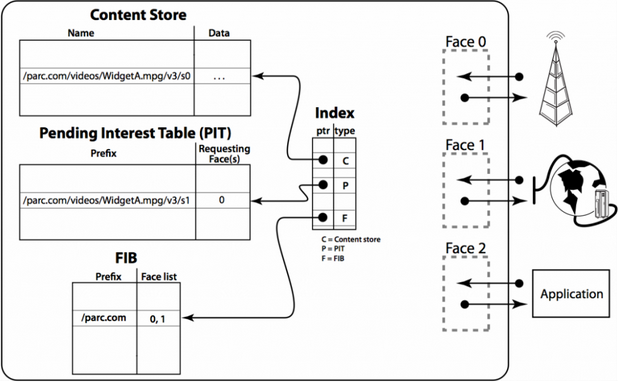
\includegraphics[scale=0.6]{chapter-2/NDNcommunication}
  \caption{Interaction of the CS, FIB and PIT data structures within a node \cite{ndn17}}
  \label{fig:NDNcommunication}
\end{figure}

In a forwarding scenario, an interest is received on Face 0 or Face 1 and a PIT entry is created if no CS match was found and no PIT already exists. If a PIT entry exists the face id is added to the entry as an incoming face. The FIB entries have outgoing faces to which interests are forwarded to, if necessary. An index keeps track of all entries in the different data structures and keeps pointers to them. If a new interest is created within the application, the interest is sent through the application face (Face 2) to the lower layers of the node for further forwarding. 

\subsection{Forwarding of an Interest}

Interests are forwarded based on the content name and the implemented strategy on all intermediate nodes. The above discussed tables are used for deciding if and how to further process the interest. The strategy is only responsible for forwarding the interests towards content sources or producers. The data coming back follows the path of the interest back to the consumer.

\vspace{5mm} %5mm vertical space

\begin{figure}[H]
  \centering
  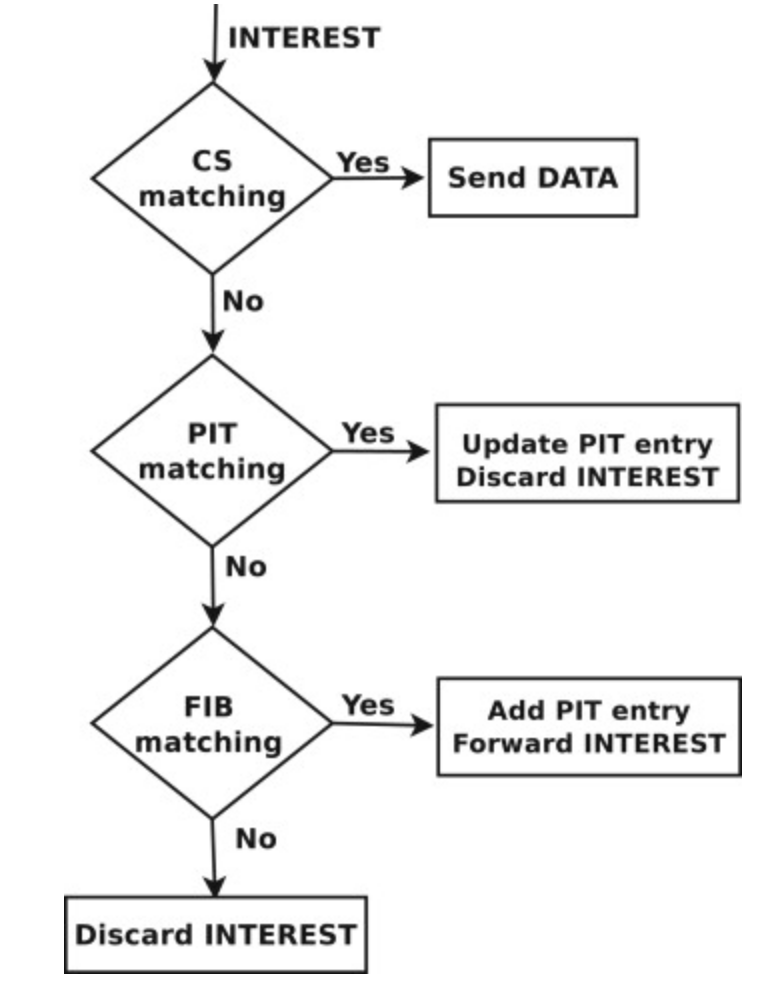
\includegraphics[scale=0.45]{chapter-2/SimpleInterestForwarding}
  \caption{Shows how the data structures are used in order to forward or discard the interest \cite{amadeo14}}
  \label{fig:SimpleInterestForwarding}
\end{figure}

\vspace{5mm} %5mm vertical space

When an interest arrives at an intermediate node the content store is checked first if the requested data has been cached already. If the interest can be satisfied by some cached data, the data message could be sent downstream towards the consumer and the interest is dropped (not further processed). If the CS has no data with the same content name as in the interest, the PIT entries are checked. If a PIT entry already exists for the interest, the node has already requested the data and is awaiting it. In that case, the incoming face(s) are added to the existing PIT entry and the interest is dropped. If a PIT entry does not exist yet and no cached data can satisfy the interest, the node checks the FIB entries for a longest prefix match, in order for the interest to be forwarded upstream towards a potential content source. If an entry is found, a new PIT entry needs to be created with the name of the interest, it's incoming face and outgoing face (from the FIB). The interest is then forwarded according to the FIB and the strategy.

\clearpage

Sending Data downstream to the original requester is straightforward and no special routing is required. The Data follows the breadcrumbs of the interest, which are left inside the PIT entries. These breadcrumbs are the incoming faces of the previously forwarded interest and serve as the outgoing faces for the data message on the way back to the requester.

\subsection{Transport and Routing}

As mentioned above the "content chunks" layer in the CCN protocol stack makes even weaker demands on the lower layers than the IP layer makes its lower layer, the Network Access Layer. It operates on unreliable, best-effort packet delivery services in potentially highly dynamic and mobile environments. Interests and Data packets are expected to get lost and/or corrupted. In CCN the strategy layer of the intermediate nodes is responsible for retransmitting the interest if within the timeout no data has been received. The strategy layer knows which outgoing faces were used and what the timeout was, therefore it is able to adjust the parameters for a retransmission. The same is true for the strategy layer of the consumer. If it does not receive any data back within a given timeframe, it will retransmit the interest, too.

\vspace{5mm} %5mm vertical space

Flow control can be managed by the consumer in terms of how many interests can be sent out before receiving the first data packet back. It is also managed on a hop-by-hop basis. Each intermediate node decides when to retransmit an interest due to loss or corrupted data coming back. The buffer for the interests is the PIT whereas the buffer for the data passing downstream to the consumers is the CS. There is no need for special congestion control techniques.

\subsection{Sequencing}

One of the big advantages in CCN over the host-to-host based TCP/IP approach is that the data in transition can be used many times by many different consumers. That leads to the problem of uniquely identifying the data in a self-explanatory way. Consumers must be able to deterministically construct a name for the data without having previously seen it. Hierarchical names that reflect the content and the organizational structure of their origin are very well suited to solve that problem. Since the naming is absolutely irrelevant for the network, applications can choose a naming that fits their need best. For example, to get the segment 34 of a video version 2 by group A of the University of Bern the name could be: \textbf{/unibe.ch/group/A/videos/introduction.mpg/\_v2/\_s32}\\
This name can be aggregated with more components if needed by the application or network. It only needs to adhere to previously specified rules.

\clearpage


\subsection{Network Security}

CCN digitally signs and encrypts the content itself and not the connection over which it travels. TCP/IP needs to secure the connections, which in turn must link the content to the server infrastructure. To trust a content object the user must fetch it from its original source making it very difficult to cache popular content and make it available to other users. For a rich and robust content-based security model the consumer must be able to assess the integrity (content is not corrupted), pertinence (what question does it answer) and provenance (who claims this is an answer). TCP/IP can only provide weak integrity through a checksum and only implicit pertinence and provenance through securing the host to host channel and therefore trusting the source and destination addresses. CCN, on the other hand, transparently provides then content name and therefore the meaning of the content which satisfies pertinence. Through public key signatures the consumer and any intermediate node can check the content's authenticity, therefore verifying integrity and satisfying provenance.

\vspace{5mm} %5mm vertical space

Content Protection and Access Control could be solved solely by encrypting the content with different keys. No trusted servers or directories would need to enforce complicated access policies on the filesystem. Expensive authentication services like SWITCH AAI could be saved. If for example, certain documents within a database should be only readable by a certain group of people these documents could be simply encrypted while still accessible to everyone. Only the people with the correct key could encrypt it and use it.
Network security is improved against many classes of network attacks. Every node can possibly (if the resources allow it) check the integrity of the data and cache it for further use. There is no single host that provides the data, therefore hiding content from consumers is very difficult.

\vspace{5mm} %5mm vertical space

DDoS attacks with data packets are not really a problem since every node can ignore unsolicited data coming in. If resources allow it, the node can simply store it in the CS and mark it as unsolicited. If space runs low on the CS these data packets will be removed first. No propagation of unsolicited data takes place since no PIT entries exist for the data. DDoS attacks, therefore, would have to be done through interests. If the prefix stays the same the PIT entry get's updated for every new interest, but no forwarding takes place. If the prefix changes constantly the strategy has many means to take action like limiting the rate of the interests with certain prefix patterns or lower prioritization of interests that result in data coming back. 

\newpage
\section{VANETs}

Vehicular ad hoc network's (VANETs) operate in very dynamic and mobile environments under possibly poor and intermittent connectivity. To the few static roadside units (RSU) there are many devices ranging from trackers and phones on pedestrians other vehicles like cars, motorcycles or drones to airplanes and satellites as shown in Figure \ref{fig:VANETecosystem}.

\vspace{5mm} %5mm vertical space

\begin{figure}[H]
  \centering
  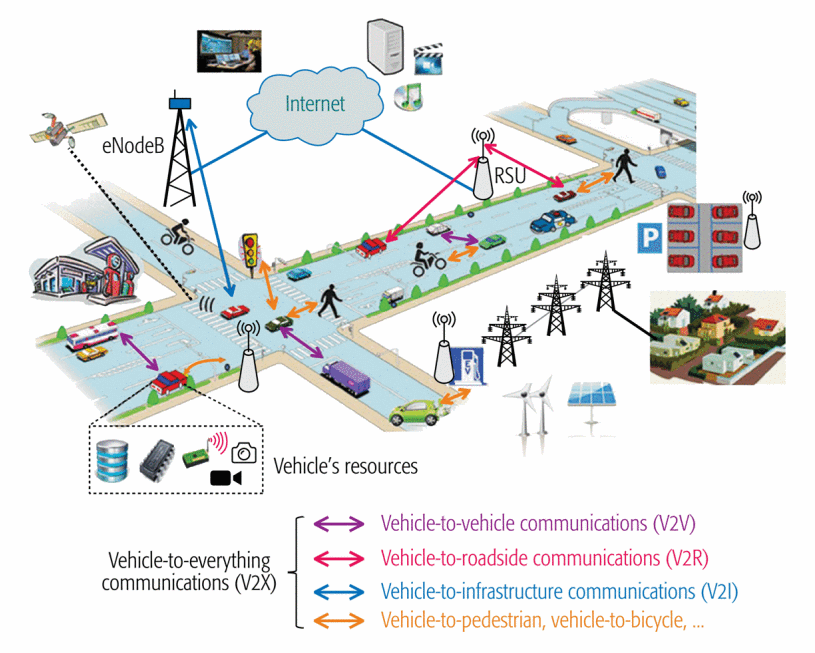
\includegraphics[scale=0.4]{chapter-2/VANETecosystem}
  \caption{Different communication agents interacting with each other through different channels}
  \label{fig:VANETecosystem}
\end{figure}

\vspace{5mm} %5mm vertical space

In such dynamic and mobile environments, the TCP/IP based approach that focuses on the source and destination and their secured connection quickly becomes a burden. Dynamic name-to-IP resolutions are difficult to do and infer a high management overhead. Keeping the connection up in urban areas where signal propagation is obstructed frequently can quickly become a challenge. Mobile IP is a workaround for this problem but does not solve the issue really. The CCN approach, on the other hand, seems to be very well suited for such ecosystems where the focus lies on the information itself (trusted road safety information for a specific area) and not on the identity of the host (other vehicles, RSU, the Internet) the data might have originated from. With in-network caching, the CCN approach also tackles the problem of poor signal strength and intermitted connectivity within a very heterogenous network system. A vehicle can store information and propagate it to an otherwise disconnected area through a \emph{store-carry-and-forward} mechanism. The multipoint to multipoint characteristics already mentioned before allows to aggregate the same interests (maps, safety warnings, road condition, congestion warnings....) and multicast the arriving data through different faces and different channels back to the consumers simultaneously.

\vspace{5mm} %5mm vertical space

There are two main routing schemes for VANETs. In the \emph{proactive} scheme, the content providers advertise periodically in order to keep the FIB entries updated with fresh routing information. In the \emph{reactive} scheme no advertisement by the content providers is done and the FIB's are populated based on interest flooding. Flooding-based discovery seems to be better suited for VANETs since periodical FIB updates on all intermediate nodes incur a high and mostly unnecessary cost on the network. An interest is able to find it's way quickly to some node having a copy of the data or the producer itself. Collision avoidance and packet suppression is done on lower layers, although packet suppression will be done in the forwarder module in ndnSIM (see chapter 3).
Caching policies in VANETs differ slightly from regular CCN use since the vehicles are moving fast into and out of regions relevant to the data. Data about possible congestion gets outdated pretty quickly so do often warnings of any kind. Further, the question arises if unsolicited data should be cached into CS and if yes, under which conditions and for how long. As mentioned before vehicles could link otherwise disconnected areas, but in that case, the data naming should be clear or that specific intent.

\vspace{5mm} %5mm vertical space

While the vehicles and devices are getting smarter and are being equipped with ever more sensors, it is expected that they will produce a huge amount of data. Most of it will be aggregated and logged, some of it will be available for distribution some of it should remain private. There are many open questions how to best support the information flow given the networks capacity. Although not originally intended by ICN the intermediate nodes could be included into in-network processing of the data like filtering useless data or aggregating redundant information.